\newpage
\thispagestyle{empty}
\ 
\newpage
\begin{chapterbox}
	\chapter[Numerical framework for simulation of turbulent iron combustion]{Numerical framework for simulation of turbulent iron combustion} \label{ch:chap2}
\end{chapterbox}
\thispagestyle{empty}
\AddToShipoutPictureBG*{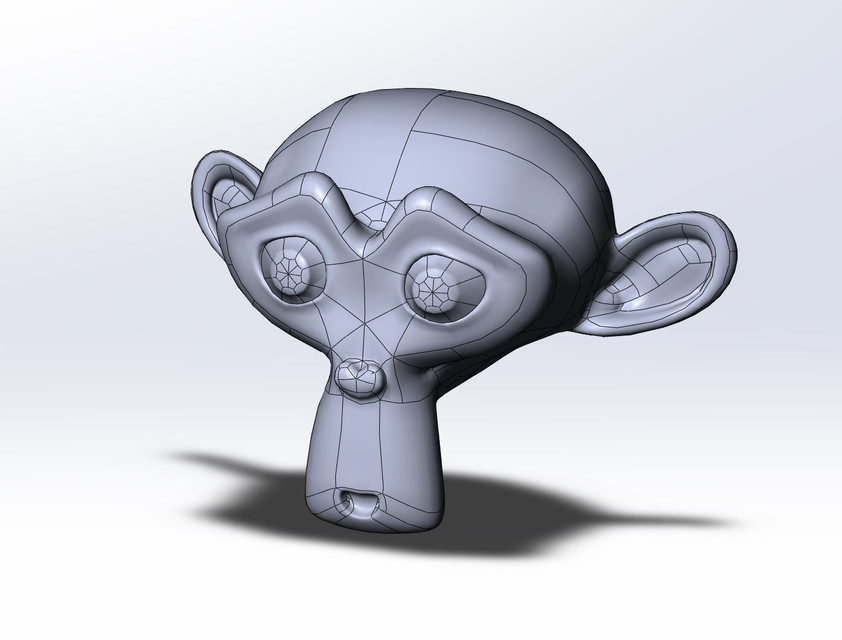
\includegraphics[height=\paperheight,trim=0cm 0 0 0cm]{Figures/chapterCovers/placeholder.jpg}}


\newpage
\thispagestyle{abstract}
\begin{abstractbox}
	\section*{Abstract}

	\lipsum[2-2]
\end{abstractbox}
\vfill
\begin{courtesybox}
	This work used the Dutch national e-infrastructure with the support of the SURF Cooperative using grant no. EINF-8301.
\end{courtesybox}

\newpage
\section{Introduction}
Citing something to show that it works \cite{Baltussen2014}. Reference to \cref{ch:chap1}. More info can be found in \cref{app:chap2}.

\section{Eulerian-Lagrangian framework}

\subsection{Gas-phase model}

\subsection{Particle model}

\subsection{Two-way coupling}

\section{Implementation}

\subsection{Direct numerical simulation in NTMIX-CHEMKIN}

\subsection{Large eddy simulation in \textit{OpenFOAM}}

\section{Validation}

\subsection{Limitations}

\section{Summary}